% Name: Apple tree
% Description: A leafy tree with a brown trunk, a round green crown, and red apples.
% Tags: tree, nature, apple, illustration

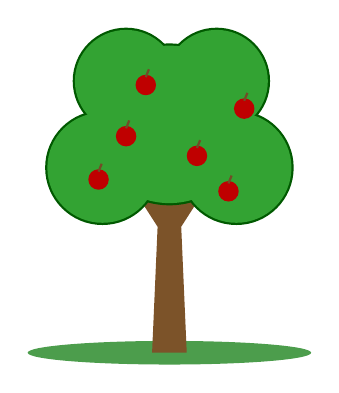
\begin{tikzpicture}
  \fill[green!45!black!70] (0,0) ellipse (1.8 and 0.15);
  % Trunk with two branches into the crown
  \fill[brown!65!black] (-0.22,0) -- (-0.15,1.6) -- (-0.6,2.3) -- (-0.45,2.38) -- (0,2.05) -- (0.45,2.4) -- (0.6,2.3) -- (0.15,1.6) -- (0.22,0) -- cycle;
  % Crown: outlines of every circle first, then the fills on top, so only the outer edge shows
  \foreach \p/\r in {{(0,2.9)/1}, {(-0.85,2.35)/0.7}, {(0.85,2.35)/0.7}, {(-0.55,3.45)/0.65}, {(0.6,3.45)/0.65}}
    \draw[green!35!black, line width=1.6pt] \p circle (\r);
  \foreach \p/\r in {{(0,2.9)/1}, {(-0.85,2.35)/0.7}, {(0.85,2.35)/0.7}, {(-0.55,3.45)/0.65}, {(0.6,3.45)/0.65}}
    \fill[green!55!black!80] \p circle (\r);
  % Apples
  \foreach \p in {(-0.9,2.2), (0.35,2.5), (-0.3,3.4), (0.95,3.1), (0.75,2.05), (-0.55,2.75)} {
    \fill[red!75!black] \p circle (0.13);
    \draw[brown!60!black, thick] \p ++(0,0.1) -- ++(0.04,0.1);
  }
\end{tikzpicture}
